\section{Implementation \& Parameters}

\begin{table}
  \caption{\label{table.size}
    Estimated size of NIPoPoWs, applied to the Bitcoin blockchain today ($\approx$450k blocks) for various values of the security parameter $m$
    setting $k = 6$.
    %and with current values for transaction count, block count,
    %coinbase size and hash output length.
  }
  \begin{tabular}{llll}
      {\bf m}  & {\bf NIPoPoW size (KB)} & {\bf \# of blocks} & {\bf
      \# of hashes}\\
      $6$   & $70$  & $108$ & $1440$  \\
      $15$  & $146$ & $231$ & $2925$  \\
      $30$  & $270$ & $426$ & $5400$  \\
      $50$  & $412$ & $656$ & $8250$ \\
      $100$ & $750$ & $1206$ & $15000$ \\
      $127$ & $952$ & $1530$ & $19050$ \\
  \end{tabular}
\end{table}



\paragraph{Interlink Optimizations}
We now discuss the exact manner in which the interlink data structure should be
hashed to provide a single hash within the coinbase transaction.  A Merkle tree
should be used to hash the interlink data structure into a single hash
\cite{KLS}.  Observe that NIPoPoWs form a single chain of various levels which
can skip certain blocks. However, it does not form a tree. Therefore, for each
block included in the proof, only a single pointer needs to be presented to
convince the Verifier. Near genesis, the pointers that need to be included
correspond to high levels; while near the most recently generated block, the
pointers correspond to low levels. One important observation is this: In the
formal construction of the proof, the highest level superchain with at least
$m$ blocks is included, and assume it is of level $\mu$. The next level
superchain, $\mu - 1$ is completely included and has an expected number of $2m$
blocks. But note that since all $\mu$-level superblocks are also $(\mu -
1)$-level superblocks, only the $\mu - 1$ level needs to be in fact included.
Among the expected $2m$ blocks of level $\mu - 1$, the last $m$ will need to be
supported by level $\mu - 2$. Using the same argument, since $(\mu - 1)$-level
superblocks are also $(\mu - 2)$ level superblocks, in expectation only $m$
blocks need to be included in level $\mu - 1$. The argument continues
inductively, until an expected number of $2m$ blocks needs to be included at
level $0$ immediately before the $\chi$ suffix.  This gives us an exact
estimation on the size of the proof: The proof will contain exactly $m
(\log(|\chain|) - \log(m))$ blocks in expectation, $m$ at each of the $\mu - 1$
levels and $2m$ at level $0$.

By organizing the interlink pointers into a Merkle tree of $\log(|\chain|)$
items, a proof-of-inclusion in the pointers Merkle tree can be provided in
$\log \log(|\chain|)$ space, noting that the $0$-level pointer need not be
included in this Merkle tree, but the genesis block needs to be. Then the root
of the pointers Merkle tree can be proved to have been included in the block
header in $\log(|\overline x|)$ using the standard Merkle tree of transactions,
where $\overline x$ is the vector of all transactions in the given block. This
makes the proof size require $\log(|\overline x|) + \log\log(|\chain|)$ hashes per
block for a total of $m (\log(|\chain|) - \log(m))(\log(|\overline x|) +
\log\log(|\chain|))$ hashes. In addition, $m (\log(|\chain|) - \log(m))$ block headers
and coinbase transactions are needed. More concretely, given that currently
$|\chain| = 464,185$, we have that $\log(|\chain|) = 18$ and $\log\log(|\chain|) =
5$.  Typically, $|\overline x| = 2000$ in the current bitcoin setting, which
makes $\log(|\overline x|) = 11$. For the $k$-suffix, only $k$ block headers need
to be included. We set $k = 6$ as is traditional in the bitcoin setting and see
that block headers are $80$ bytes and hash outputs are $32$ bytes. However, we
note that block headers do not need to include the previous block header hash
for the $k$-suffix, as each previous block header hash can be calculated by the
Verifier, limiting header sizes to $48$ bytes for the $k$ last blocks.
Furthermore, the $k$-suffix does not require the presentation of the coinbase
transaction data. These are also true for the $2m$ blocks in $\overline \Pi[0]$.
Note also that for the proof prefix $\overline \Pi$, the coinbase transaction
hash need not be included: It can be evaluated by the Verifier when building
the Merkle tree during the proof-of-inclusion. Similarly, the root of the
pointers Merkle tree can be omitted from the coinbase transaction data when
transmitting the proof. Additionally, the leaf of the pointers Merkle tree can
also be omitted, as it can be obtained by the Verifier by simply hashing the
previous block in the proof. In fact, no block ids need to be transmitted at
all, as they can all be built from the Verifier starting from the knowledge of
Genesis.

From these observations, we estimate our scheme's proof sizes  for various parameterizations of $m$ in Table~\ref{table.size}.


\subsection{Choosing Secure Parameters}
In order to determine concrete values for the security parameter $m$, we now
turn our attention to a particular adversarial strategy of interest and analyze
its probability of success under specific conditions. It is important to keep
in mind that this adversarial strategy is only one possible strategy and an
advanced adversary can perform more sophisticated attacks. However, the fact
that this attack is reasonable and possible to simulate allows us to extract
specific values for $m$.
The attack is an extension of the stochastic processes originally described in
\cite{bitcoin} and further explored in \cite{rosenfeld}.

The experiment works as follows: Initially, the value $m$ is fixed and some
adversarial computational power percentage $q$ over the total network
computational power is chosen. $k$ is chosen based on $q$ according to Nakamoto
\cite{bitcoin}. The number of blocks $y$ during which parallel mining will
occur is also fixed. Then the experiment begins with the adversary and the
honest parties sharing a common blockchain which ends in block $B$. As soon as
$B$ is mined, the adversary starts mining in secret and in parallel with the
honest parties on his own private fork on top of $B$. She ignores the honest
chain and does not publish her private fork, so that the two chains remain
disjoint after $B$. As soon as $y$ blocks have been mined in total, the
adversary attempts a double spend by creating two conflicting transactions
which are committed to an honest block and an adversarial block respectively on
top of each current chain. Finally, the adversary mines $k$ blocks on top of
the double spending transaction within her private chain. As soon as these $k$
blocks have been mined, she publishes her private chain in an attempt to
overcome the honest chain.

Based on the above experiment, we measure the probability of success of the
adversary. We experiment
with various values of $m$ for $y = 100$, indicating $100$ blocks of secret
parallel mining. We make the simplifying assumption that honest party
communication is perfect and immediate, meaning that all honest party rounds
that are successful are also uniquely successful. We ran $1,000,000$ Monte
Carlo executions \footnote{The URL to the GitHub repository of this
MIT-licensed experiment has been redacted for anonymity and will be provided in
the proceedings version of this paper.} of the experiment for each value of $m$
from $1$ to $30$. We ran the simulation for values of computational power
percentage $q = 0.1$, $q = 0.2$ and $q = 0.3$. The results are plotted in
Figure~\ref{fig.nipopow-attack-experiment}.

\begin{figure}
    \caption{\label{fig.nipopow-attack-experiment}
        Simulation results for a private mining attacker with $q \in \{0.1,
        0.2, 0.3\}$ computational power, suffix security $k$ according to
        Nakamoto and parallel mining parameter $y = 100$. Probabilities are
        plotted on a logarithmic scale. The threshold probability of
        \cite{bitcoin} is indicated by the horizontal line.
    }
    \centering
    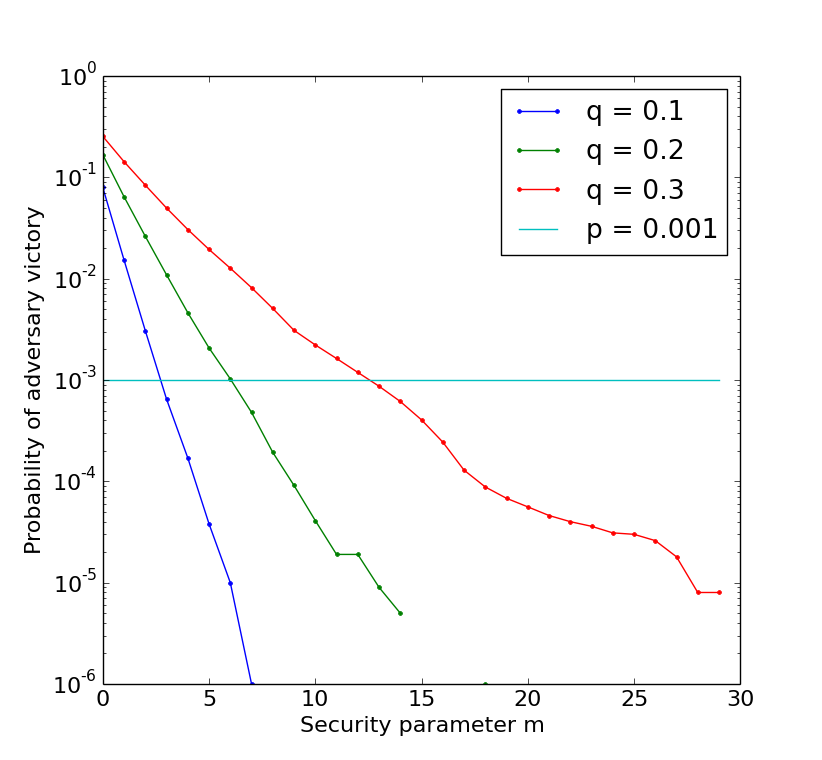
\includegraphics[width=\columnwidth,keepaspectratio]{figures/nipopow-attack-experiment.png}
\end{figure}

Based on this data, we conclude that $m = 5$ is sufficient to achieve a $0.001$
probability of failure against an adversary with $10\%$ mining power. To secure
against a powerful adversary who controls more than $30\%$ of the network's
mining power, a choice of $m = 15$ is needed.
